\documentclass{beamer}
\usepackage[latin1]{inputenc}
\usepackage{tikz}
\usepackage{tikzscale}
\usepackage{pgfplots}
\pgfplotsset{compat=1.15}
\pgfplotsset{
  /pgfplots/xlabel near ticks/.style={
     /pgfplots/every axis x label/.style={
        at={(ticklabel cs:0.5)},anchor=near ticklabel
     }
  },
  /pgfplots/ylabel near ticks/.style={
     /pgfplots/every axis y label/.style={
        at={(ticklabel cs:0.5)},rotate=90,anchor=near ticklabel}
     }
  }
\usepackage[algosection,  linesnumbered]{algorithm2e}
\usepackage{enumerate}
\usepgfplotslibrary{groupplots}
\usepgfplotslibrary{colorbrewer}
\usepackage{filecontents}
\usepackage{adjustbox}

\setbeamertemplate{itemize items}[circle]

\usetheme{Dresden}
\usecolortheme{beaver}
\title[]{Numerical Solutions to Loewner's Equation and Applications}
\author{Dolica Akello-Egwel}
\date{September 4th 2018}

\begin{document}

% Title Page
\begin{frame}
\titlepage
\end{frame}

% Introducing Loewner's Equation
\begin{frame}{Loewner's Equation}
\begin{adjustbox}{max totalsize={.9\textwidth}{.7\textheight},center}
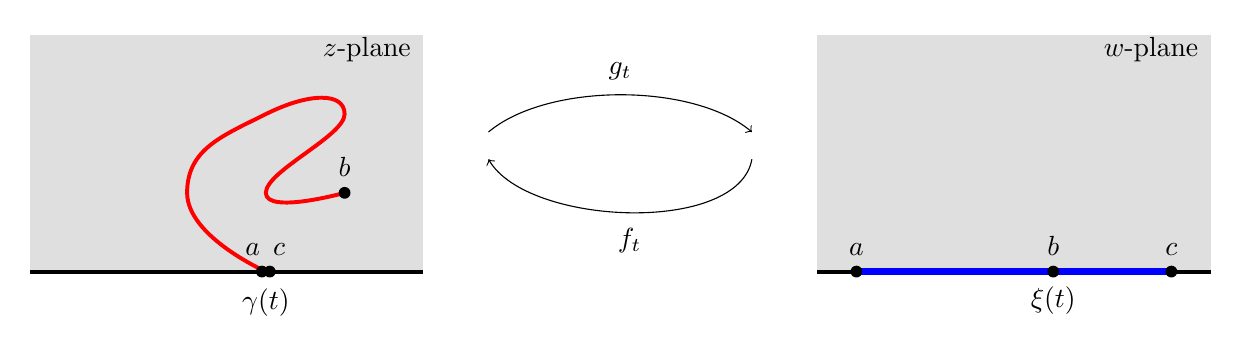
\begin{tikzpicture}
\fill [gray!25] (-3,0) rectangle (2,3);
    \draw [line width=0.5mm,red] plot [smooth, tension=1] coordinates {(0,0) (-1,1) (0,2) (1,2) (0,1) (1,1)};
    \draw [line width=0.5mm, black]  (-3,0) -- (2,0);
    \draw (2,3) node[below=0.5em,left=1pt] {$z$-plane};
    \draw (0,0) node[below=1mm] {$\gamma(t)$};
    \draw (0,0) node[xshift=-0.05cm,circle,black,inner sep=0pt,minimum size=1.5mm,fill,label=$a \ \ $]{};
    \draw (0,0) node[xshift=0.05cm,circle,black,inner sep=0pt,minimum size=1.5mm,fill,label=$\ \ c$]{};
    \draw (1,1)  node[circle,inner sep=0pt, minimum size=1.5mm,fill,label=$b$]{};
    \node[anchor=east,xshift=5cm,circle] at (-2,1.6) (Start) {};
    \node[anchor=west,xshift=5cm,circle] at (1,1.6) (End) {};
    \draw [->,out=40,in=140,looseness=0.75] (Start.north) to node[above=2pt]{$g_t$}  (End.north);
    \draw [->,out=260,in=300,looseness=0.75] (End.south) to node[below=2pt]{$f_t$}  (Start.south);
    \fill [gray!25,xshift=10cm] (-3,0) rectangle (2,3);
    \draw [line width=0.5mm, black,xshift=10cm]  (-3,0) -- (2,0);
    \draw [line width=0.8mm, blue,xshift=10cm]  (-2.5,0) -- (1.5,0);
    \draw (-2.5,0) node[circle,black,inner sep=0pt,xshift=10cm,minimum size=1.5mm,fill,label=$a$]{};
    \draw (0,0) node[circle,black,inner sep=0pt,xshift=10cm,minimum size=1.5mm,fill,label=$b$]{};
    \draw (1.5,0)  node[xshift=10cm,circle,inner sep=0pt, minimum size=1.5mm,fill,label=$c$]{};
    \draw (0,0) node[xshift=10cm,below=2] {$\xi(t)$};
    \draw (2,3) node[xshift=10cm,below=0.5em,left=1pt] {$w$-plane};
\end{tikzpicture}

\end{adjustbox}

$$g_t = \frac{2}{g - \xi(t)}, \quad\quad\quad g_0(z) = z$$

Applications:
\begin{itemize}
\item Growth of cracks
\item Formation of stream networks
\item Percolation/self-avoiding walks
\end{itemize}
\end{frame}

% Project Objectives
\begin{frame}{Project Objectives}
    \begin{enumerate}[(i)]
    \item Forward problem: Numerically solve Loewner's equation given $\xi(t)$ to find trace
    \item Inverse problem: Given the trace, find the driving function $\xi(t)$
    \item Two-trace evolutions
    \item Evolution in a wedge geometry
\end{enumerate}
\end{frame}

% The Forward Problem
\begin{frame}{The Forward Problem}
    \begin{itemize}
        \item Objective: Given a driving function $\xi(t)$, find the trace.
        \item Numerical approach: Use finite differences, follow a technique described by Kager et al. (2004).
    \end{itemize}

    \begin{equation*}
        \dot{g_t} \simeq \frac{g_t - g_{t - \delta t}}{\delta t} = \frac{2}{g_{t - \delta t} - \xi(t - \partial t)}
    \end{equation*}

    \begin{itemize}
        \item $\Rightarrow$ Determine $g_{t - \delta t}$ by solving a quadratic
        \item  Find $g_{t - 2\delta t},g_{t - 3\delta t} \dots \Rightarrow$ Find $g_0$
    \end{itemize}

\end{frame}

% The Forward Problem - Algorithm (2.1 From Report)
\begin{frame}{The Forward Problem: Algorithm}
\begin{algorithm}[H]
    \footnotesize
    \SetKwFunction{Lin}{Linspace}
    \SetKwFunction{Sol}{SolveQuadratic}
    \SetKwFunction{Com}{complex}

        \KwIn{$T_0$, $T_F$, $N_{\text{inner}}$, $N_{\text{outer}}$, $\xi(t)$}
        \KwOut{An array $z[\thinspace]$ containing $N_{\text{outer}}$ values of $g_0$}

        $ N_{\text{total}} \leftarrow (N_{\text{outer}} - 1)*N_{\text{inner}}$ \\
        $ t[\thinspace] \leftarrow \Lin(T_0,T_F,N_{\text{total}})$ \\
        $ \delta t \leftarrow t_1$ \\

        $ z[\thinspace] \leftarrow \Com[N_{\text{outer}}] $ \\
        $ z_0 \leftarrow \xi(T_0) $ \\

        \For{$ i \leftarrow 1 \enspace \KwTo \enspace N_{\text{outer}} - 1$}{
            $ g_\text{J} \leftarrow \xi(T_i) $ \\
            \For{$ j \leftarrow i*N_{\text{inner}} \enspace \KwTo \enspace 0$}{
                $ g_\text{j - 1} \leftarrow \Sol((g_j - g_{j-1})(g_{j-1} - \xi(t_{j-1})) - 2\delta t = 0) $
         }
        $ z_i \leftarrow g_0 $
 }
\nl\KwRet{$z[\thinspace]$}
\end{algorithm}
\end{frame}

% Constant Driving
\begin{frame}{Constant Driving - $\xi(t) = 0$}
\begin{adjustbox}{max totalsize={\textwidth}{\textheight}}
\begin{tikzpicture}
    \begin{axis}[
            name=mygraph,
            ymin=0,
            xmin=-0.5,
            xmax=0.5,
            xlabel={$\operatorname{Re}(z)$},
            ylabel={$\operatorname{Im}(z)$},
            height=\axisdefaultheight,
            width=\axisdefaultwidth,
            ylabel near ticks,
            tick align=inside,
            tick pos=left,
            xmajorgrids,
            x grid style={gray!25},
            ymajorgrids,
            y grid style={gray!25},
            cycle list name=exotic,
            ] % enabling scale only axis destroys this plot
                \addplot+[line width=2pt] table [col sep=space,mark=none,smooth] {Data/SingleTrace/Forward/0-0-25-1000-10.dat};
                \addplot+[line width=2pt] table [col sep=space,mark=none,smooth] {Data/SingleTrace/Forward/0-0-16-1000-10.dat};
                \addplot+[line width=2pt] table [col sep=space,mark=none,smooth] {Data/SingleTrace/Forward/0-0-9-1000-10.dat};
                \addplot+[line width=2pt] table [col sep=space,mark=none,smooth] {Data/SingleTrace/Forward/0-0-4-1000-10.dat};
                \addplot+[line width=2pt] table [col sep=space,mark=none,smooth] {Data/SingleTrace/Forward/0-0-1-1000-10.dat};
                \draw[red,dotted,very thick] (-0.5,2) -- (0,2);
                \node[black,right=5pt] at (axis cs:0,2){$T_F = 1$};
                \draw[red,dotted,very thick] (-0.5,4) -- (0,4);
                \node[black,right=5pt] at (axis cs:0,4){$T_F = 4$};
                \draw[red,dotted,very thick] (-0.5,6) -- (0,6);
                \node[black,right=5pt] at (axis cs:0,6){$T_F = 9$};
                \draw[red,dotted,very thick] (-0.5,8) -- (0,8);
                \draw[red,dotted,very thick] (-0.5,10) -- (0,10);
                \node[black,right=5pt] at (axis cs:0,8){$T_F = 16$};
                \node[black,right=5pt,] at (axis cs:0,10){$T_F = 25$};
                \fill (0,10) circle[radius=2pt];
                \fill (0,8) circle[radius=2pt];
                \fill (0,6) circle[radius=2pt];
                \fill (0,4) circle[radius=2pt];
                \fill (0,2) circle[radius=2pt];
            \end{axis}
    \node[xshift=75pt] at ($(mygraph.south east)!0.5!(mygraph.north east)$){Exact solution:};
    \node[xshift=75pt,yshift=-15pt] at ($(mygraph.south east)!0.5!(mygraph.north east)$){$z_c(t) = 2i \sqrt{T_F}$};
\end{tikzpicture}

\end{adjustbox}
\end{frame}

% Linear Driving
\begin{frame}{Linear Driving - $\xi(t) = t$}
    \begin{tabular}{cc}
\begin{adjustbox}{max totalsize={.3\textwidth}{.9\textheight}}
\begin{tikzpicture}
    \begin{groupplot}[
            group style={
                group name=left plots,
                group size=1 by 2,
                vertical sep = 45pt},
            height=0.4\textwidth,
            width=0.4\textwidth,
            clip mode=individual,
            tick align=inside,
            tick pos=left,
            xmajorgrids,
            x grid style={gray!25},
            ymajorgrids,
            y grid style={gray!25},
            scale only axis]
        \nextgroupplot[ylabel={$\operatorname{Im}(z)$},xlabel={$\operatorname{Re}(z)$},ymin=0,legend pos = south east,]
            \addplot[orange,line width=2pt] table [col sep=space,mark=none,smooth] {Data/SingleTrace/Forward/1-0-25-1000-10.dat};
            \addplot[black,dash pattern=on 5pt off 3pt,line width=2pt] table [col sep=space,smooth] {Data/SingleTrace/ExactForward/1-0-25-1000.dat};
            \legend{{Numerical},{Exact}};
        \nextgroupplot[xlabel={$N_{\text{inner}}$},ylabel={Root-Mean-Square Error},]
            \addplot[color=green!70!black,mark=square*,line width=0.5mm] table [col sep=space] {Data/SingleTrace/RootMeanSquared/Forward/1-RMS.dat};
    \end{groupplot}
\end{tikzpicture}


\end{adjustbox}
\begin{adjustbox}{max totalsize={.7\textwidth}{.9\textheight}}
\begin{tikzpicture}
    \begin{groupplot}[
            group style={
                group name=left plots,
                group size=1 by 1,
                vertical sep = 50pt,
                y descriptions at=edge left},
            height=160pt,
            width=0.9\textwidth,
            xmin=-50,
            ymin=0,
            xmax=2100,
            ylabel={$\operatorname{Im}(z)$},
            xlabel={$\operatorname{Re}(z)$},
            ylabel near ticks,
            tick align=inside,
            tick pos=left,
            xmajorgrids,
            x grid style={gray!25},
            ymajorgrids,
            y grid style={gray!25},
            ]
        \nextgroupplot[]
            \addplot table [col sep=space,mark=none,smooth] {Data/SingleTrace/ExactForward/1-PHI-0point00314-3point13845-1000.dat};
    \end{groupplot}
    \node[yshift=65pt,anchor=west,xshift=-15pt] at ($(left plots c1r1.north east)!0.9!(left plots c1r1.north west)$){\textbf{Exact Solutions:}};
    \node[yshift=47pt,anchor=west,xshift=-15pt] at ($(left plots c1r1.north east)!0.9!(left plots c1r1.north west)$){Explicit: $z_c(t) = 2 - 2 \phi_t \cot \phi_t + 2i \phi_t$};
    \node[yshift=35pt,anchor=west,xshift=-15pt] at ($(left plots c1r1.north east)!0.9!(left plots c1r1.north west)$){Implicit: $z_c(t) = t - 2 \ln (2 - z_c(t)) + 2 \ln(2)$};
\end{tikzpicture}


\end{adjustbox}
\end{tabular}
\end{frame}

% Square-Root Driving
\begin{frame}{Square-Root Driving}
\begin{adjustbox}{max totalsize={\textwidth}{\textheight}}
\begin{tikzpicture}
    \begin{groupplot}[ % This is actually kappa
            group style={
                group name=left plots,
                group size=1 by 2,
                vertical sep = 45pt,
                },
            ymin=0,
            width=0.9\textwidth,
            xlabel near ticks,
            height=135pt,
            tick align=inside,
            tick pos=left,
            xmajorgrids,
            x grid style={gray!30},
            ymajorgrids,
            cycle list/Dark2,
            y grid style={gray!30}
            ]
        \nextgroupplot[title={\large ${\xi(t) = 2\sqrt{\kappa(1 - t)}}$},xlabel={$\operatorname{Re}(z)$},ylabel={$\operatorname{Im}(z)$},scale only axis,xmax=2.5,legend pos=north east,]
            \addplot+[line width=0.3mm] table [col sep=space,mark=none,smooth] {Data/SingleTrace/TranslatedForward/10-1point5-0-1-1000-500.dat};
            \addplot+[line width=0.3mm] table [col sep=space,mark=none,smooth] {Data/SingleTrace/TranslatedForward/10-2point5-0-1-1000-500.dat};
            \addplot+[line width=0.3mm] table [col sep=space,mark=none,smooth] {Data/SingleTrace/TranslatedForward/10-3point5-0-1-1000-500.dat};
            \addplot+[line width=0.3mm] table [col sep=space,mark=none,smooth] {Data/SingleTrace/TranslatedForward/10-4point5-0-1-1000-500.dat};
            \addplot+[line width=0.3mm] table [col sep=space,mark=none,smooth] {Data/SingleTrace/TranslatedForward/10-5point5-0-1-1000-500.dat};
            \addplot+[line width=0.3mm] table [col sep=space,mark=none,smooth] {Data/SingleTrace/TranslatedForward/10-6point5-0-1-1000-500.dat};
            \addplot+[line width=0.3mm] table [col sep=space,mark=none,smooth] {Data/SingleTrace/TranslatedForward/10-7point5-0-1-1000-500.dat};
            \addplot+[line width=0.3mm] table [col sep=space,mark=none,smooth] {Data/SingleTrace/TranslatedForward/10-8point5-0-1-1000-500.dat};
            \addplot+[red,line width=0.3mm] table [col sep=space,mark=none,smooth] {Data/SingleTrace/TranslatedForward/10-9point5-0-1-1000-500.dat};
            \legend{$\kappa=1.5$,$\kappa=2.5$,$\kappa=3.5$,$\kappa=4.5$,$\kappa=5.5$,$\kappa=6.5$,$\kappa=7.5$,$\kappa=8.5$,$\kappa=9.5$}
    \end{groupplot}
\end{tikzpicture}

\end{adjustbox}
\end{frame}

% Non-Smooth Driving
\begin{frame}{Non-Smooth Driving}
\begin{adjustbox}{max totalsize={\textwidth}{\textheight}}
\begin{tikzpicture}
    \begin{groupplot}[
            group style={
                horizontal sep = 45pt,
                group name=left plots,
                group size=2 by 1,
            },
            height=0.7\textwidth,
            width=0.7\textwidth,
            tick align=inside,
            xlabel near ticks,
            ylabel near ticks,
            tick pos=left,
            xmajorgrids,
            x grid style={gray!25},
            ymajorgrids,
            y grid style={gray!25},
            ]
        \nextgroupplot[title={$\xi(t) = \lfloor t \rfloor$},ymin=0,xlabel={$\operatorname{Re}(z)$},ylabel={$\operatorname{Im}(z)$},legend pos=south east]
            \addplot[color=black,line width=0.4mm] table [mark=none,smooth] {Data/SingleTrace/Forward/1-0-25-1000-10.dat};
            \addplot[color=red,line width=0.4mm] table [mark=none,smooth] {Data/SingleTrace/Forward/12-0-25-1000-10.dat};
            \legend{$\xi(t) = t$,$\xi(t) = \lfloor t \rfloor$};
        \nextgroupplot[extra x ticks={0.5},ymin=0,ymax=11,xlabel={$\operatorname{Re}(z)$},ylabel={$\operatorname{Im}(z)$},title={$\xi(t) = \lfloor t \rfloor \mod 2$}]
            \draw[black,dotted,very thick] (0.5,0) -- (0.5,11);
            \addplot+[,line width=0.4mm] table [mark=none,smooth] {Data/SingleTrace/Forward/13-0-25-1000-10.dat};
    \end{groupplot}
\end{tikzpicture}

\end{adjustbox}
\end{frame}

\end{document}
